\documentclass[main.tex]{subfiles}
\begin{document}
\subsection{化学势的引入}
热力学能$U$作为特性函数,是以熵$S$、体积$V$和各组分的摩尔数$n_1,n_2,\cdots$为特征变量的函数。以下简记各组份的摩尔数为$\left\{n_i\right\}$。热力学能作为特性函数的全微分是
\[\mathrm{d}U=\left.\frac{\partial U}{\partial S}\right|_{V,\left\{n_i\right\}}\mathrm{d}S+\left.\frac{\partial U}{\partial V}\right|_{S,\left\{n_i\right\}}\mathrm{d}V+\sum_i\left.\frac{\partial U}{\partial n_i}\right|_{S,V,\left\{n_{j\neq i}\right\}}\mathrm{d}n_i\]
与由热力学第一、二定律得到的式子
\begin{align}
    dU=TdS-pdV+\sum_i\mu_idn_i\quad\text{(可逆过程)}\label{eq:thermodynamic_relations_U}
\end{align}
比较,得
\[T=\left.\frac{\partial U}{\partial S}\right|_{V,\left\{n_i\right\}},\quad-p=\left.\frac{\partial U}{\partial V}\right|_{S,\left\{n_i\right\}},\quad\mu_i\equiv\left.\frac{\partial U}{\partial n_i}\right|_{S,V,\left\{n_{j\neq i}\right\}}\]
其中$T$是温度,$p$是压强,$\mu_i$是此处引入的,表示由于组份$i$的分子数变化$dn_i$所造成的混合物体系热力学能的变化,称为组份$i$在混合物中的\CJKunderdot{化学势}(chemical potential)。由微分关系可进一步导出其他几个特性函数的微分式(可逆过程):
\begin{align}    \mathrm{d}H & =T\mathrm{d}S+V\mathrm{d}p+\sum_i\mu_i\mathrm{d}n_i\label{eq:thermodynamic_relations_H}  \\
                 \mathrm{d}A & =-S\mathrm{d}T-p\mathrm{d}V+\sum_i\mu_i\mathrm{d}n_i\label{eq:thermodynamic_relations_A} \\
                 \mathrm{d}G & =-S\mathrm{d}T+V\mathrm{d}p+\sum_i\mu_i\mathrm{d}n_i\label{eq:thermodynamic_relations_G}
\end{align}
其中$H$是焓,$A$是亥姆霍兹自由能,$G$是吉布斯自由能。它们的定义是
\begin{align}
    H & =U+pV\label{eq:def_of_H}    \\
    A & =U-TS\label{eq:def_of_A}    \\
    G & =U+pV-TS\label{eq:def_of_G}
\end{align}

由式\eqref{eq:thermodynamic_relations_H}至\eqref{eq:thermodynamic_relations_G}可见,化学势恰好同时是其他几个特性函数对组份的偏导数:
\begin{equation}
    \label{eq:chemical_potential_as_partial_molar_characteristic_functions}
    \mu_i=\left.\frac{\partial U}{\partial n_i}\right|_{S,V,\left\{n_{j\neq i}\right\}}=\left.\frac{\partial H}{\partial n_i}\right|_{S,p,\left\{n_{j\neq i}\right\}}=\left.\frac{\partial A}{\partial n_i}\right|_{T,V,\left\{n_{j\neq i}\right\}}=\left.\frac{\partial G}{\partial n_i}\right|_{T,p,\left\{n_{j\neq i}\right\}}
\end{equation}

我们常常考虑体系的平衡状态由$T$、$p$和$\left\{n_i\right\}$确定的过程。此时应考虑的特性函数是吉布斯自由能$G\left(T,p,\left\{n_i\right\}\right)$。由吉布斯自由能的定义$G\equiv U-TS+pV$,
\begin{align*}
    \mathrm{d}G & =\mathrm{d}U-T\mathrm{d}S-S\mathrm{d}T+p\mathrm{d}V+V\mathrm{d}p                                       & \text{(} & \text{微分规则)}                                    \\
                & =T\mathrm{d}S-p\mathrm{d}V+\sum_i\mu_i\mathrm{d}n_i-T\mathrm{d}S-S\mathrm{d}T+\mathrm{d}V+V\mathrm{d}p & \text{(} & \text{代入式\eqref{eq:thermodynamic_relations_U})} \\
                & =\sum_i\mu_i\mathrm{d}n_i-S\mathrm{d}T+V\mathrm{d}p                                                    &
\end{align*}
与式\eqref{eq:thermodynamic_relations_G}比较得:
\begin{equation}\label{eq:partial_diff_of_G}
    S=\left.\frac{\partial G}{\partial T}\right|_{p,\left\{n_i\right\}},\quad V=\left.\frac{\partial G}{\partial p}\right|_{T,\left\{n_i\right\}},\quad\mu_i=\left.\frac{\partial G}{\partial n_i}\right|_{T,p,\left\{n_{j\neq i}\right\}}
\end{equation}
通过类似的方法,可以针对其他特性函数得出类似的关系并再一次确认式\eqref{eq:chemical_potential_as_partial_molar_characteristic_functions}。若进一步对共享同一量的偏导数求交叉偏导数,可得到一系列Maxwell关系:
\begin{equation}\label{eq:Maxwell_relations}
    \begin{aligned}
        \left.\frac{\partial S}{\partial p}\right|_{T,\left\{n_i\right\}}                & =-\left.\frac{\partial V}{\partial T}\right|_{p,\left\{n_i\right\}}               \\
        \left.\frac{\partial S}{\partial n_i}\right|_{T,p,\left\{n_{j\neq i}\right\}}    & =-\left.\frac{\partial\mu_i}{\partial T}\right|_{p,\left\{n_i\right\}}            \\
        \left.\frac{\partial V}{\partial n_i}\right|_{T,p,\left\{n_{j\neq i}\right\}}    & =\left.\frac{\partial \mu_i}{\partial p}\right|_{T,\left\{n_i\right\}}            \\
        \left.\frac{\partial\mu_i}{\partial n_j}\right|_{T,p,\left\{n_{k\neq j}\right\}} & =\left.\frac{\partial\mu_j}{\partial n_i}\right|_{T,p,\left\{n_{k\neq i}\right\}}
    \end{aligned}
\end{equation}

将式\eqref{eq:partial_diff_of_G}重新代入吉布斯自由能的定义中可得:
\[
    U=G-T\left.\frac{\partial G}{\partial T}\right|_{p,\left\{n_i\right\}}-p\left.\frac{\partial G}{\partial p}\right|_{T,\left\{n_i\right\}}
\]
其他热力学函数也可由$G$导出:
\begin{align}
    H & =G-T\left.\frac{\partial G}{\partial T}\right|_{p,\left\{n_i\right\}} \\
    A & =G-p\left.\frac{\partial G}{\partial p}\right|_{T,\left\{n_i\right\}}
\end{align}

\subsection{偏摩尔量}
作为广延量的热力学函数$Z=Z\left(X,Y,\left\{n_i\right\}\right)$,在恒定$X$、$Y$下是$\left\{n_i\right\}$的一次齐函数,即
\[Z\left(X,Y,\left\{\lambda n_i\right\}\right)=\lambda Z\left(X,Y,\left\{n_i\right\}\right),\quad\forall\lambda\in\mathbb{R}\]
由齐函数的欧拉定理\ref{thm:Euler_theorem_for_homogeneous_function},在恒定$X$、$Y$下$Z$总能写成
\[Z=\sum_i n_i\left.\frac{\partial Z}{\partial n_i}\right|_{X,Y,\left\{n_{j\neq i}\right\}}=\sum_i n_i z_i\]
其中
\[z_i\equiv\left.\frac{\partial Z}{\partial n_i}\right|_{X,Y,\left\{n_{j\neq i}\right\}}\]
称偏摩尔$Z$(partial molar $Z$),是$Z$关于组份$i$的偏摩尔量(partial molar quantity)。由齐函数定义易推出,在恒定$X$、$Y$下,$z_i$是$\left\{n_i\right\}$的零次齐函数。特别地,当$\lambda=1/\sum_i n_i=1/n$时有
\[z_i\left(X,Y,\left\{\lambda x_i\right\}\right)=z_i\left(X,Y,\left\{n_i\right\}\right)\]
其中$x_i\equiv n_i/n$是组份$i$在体系中的摩尔分数,$n\equiv\sum_i n_i$。上述结论相当于说,偏摩尔量都是强度量。

延续上一段文字的符号设定,$Z$直接被$n$除所得到的量叫平均摩尔$Z$(mean molar $Z$)或简称摩尔$Z$(molar $Z$),是体系的$Z$的摩尔量(molar quantity),记作
\[Z_\text{m}\equiv\frac{Z}{n}\]

特别地,化学势是各特性函数的偏摩尔量。以吉布斯自由能为例,有$G=\sum_i n_i\mu_i$。对其求微分得
\[\mathrm{d}G=\sum_i\left(n_i\mathrm{d}\mu_i+\mu_i\mathrm{d}n_i\right)\]
与式\eqref{eq:thermodynamic_relations_G}比较得
\begin{equation}\label{eq:Gibbs-Duhem eq.}
    -S\mathrm{d}T+V\mathrm{d}p-\sum_i n_i\mathrm{d}\mu_i=0
\end{equation}
称为吉布斯--杜亥姆方程(Gibbs--Duhem equation)。在恒定$T$、$p$下,上式变为
\[\sum_i n_i\mathrm{d}\mu_i=0\]
由上述关于$Z$的一般讨论不难推出,一般地,在恒定$X$、$Y$下,总有
\begin{equation}\label{eq:generalized_Gibbs_Duhem eq.}
    \sum_i n_i \mathrm{d}z_i=0
\end{equation}

留意到,Maxwell关系式\eqref{eq:Maxwell_relations}中含有偏摩尔量,即
\[s_i=-\left.\frac{\partial\mu_i}{\partial T}\right|_{p,\left\{n_i\right\}},\quad v_i=\left.\frac{\partial\mu_i}{\partial p}\right|_{T,\left\{n_i\right\}}\]

\subsection{偏摩尔量的实验测量原理}
实验上,我们往往只能测量一个多组份体系的摩尔量$Z_\text{m}=Z_\text{m}\left(X,Y,\left\{n_i\right\}\right)$随某组份$i$在恒定$X$、$Y$下的变化。以下推算,使得我们能够通过$Z_\text{m}$对$x_i$的曲线得出$z_i$。

在恒定$X$、$Y$下,$Z=n Z_\text{m}$,对其进行微分有
\[\mathrm{d}\left(nZ_\text{m}\right)=n\mathrm{d}Z_\text{m}+Z_\text{m}\mathrm{d}n\]
对$n=\sum_i n_i$进行微分有
\[\mathrm{d}n=\sum_i\mathrm{d}n_i\]
上列两式联立起来有
\[n\mathrm{d}Z_\text{m}+Z_\text{m}\sum_i \mathrm{d}n_i=\sum_i z_i\mathrm{d}n_i\]
利用该式求关于$n_i$的偏导(即保持$\left\{n_{j\neq i}\right\}$恒定),得到
\begin{align*}
                    & n\left.\frac{\partial Z_\text{m}}{\partial n_i}\right|_{X,Y,\left\{n_{j\neq i}\right\}}+Z_\text{m}=z_i+\sum_{j\neq i}z_j\left.\frac{\partial n_j}{n_i}\right|_{n_{j\neq i}} \\
    \Leftrightarrow & \left(1-x_i\right)\left.\frac{\partial Z_\text{m}}{\partial x_i}\right|_{X,Y,\left\{n_{j\neq i}\right\}}+Z_\text{m}=z_i
\end{align*}

利用这一结论,偏摩尔量$z_i$就能由$Z_\text{m}$对$x_i$的曲线数据,如图\ref{fig:meas_partial_molar_quant}所示般得出。

\begin{figure}[h]
    \centering
    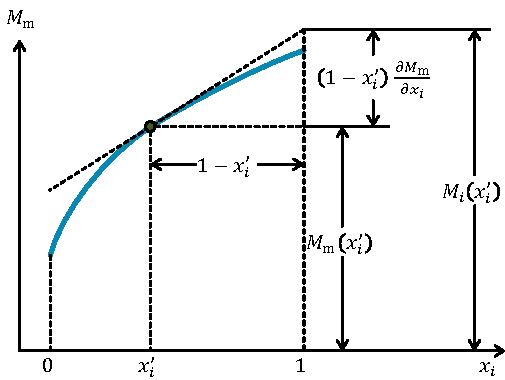
\includegraphics{../images/meas_partial_molar_quant.pdf}
    \caption{从摩尔量曲线求偏摩尔量的“截距法”。}
    \label{fig:meas_partial_molar_quant}
\end{figure}

《物理化学》\S 4.3中的“偏摩尔量的求法”之“3.截距法”介绍了上述方法对于双组份混合物的特例。

\end{document}